\documentclass[11pt]{article}

%%%%%%%%%%%%%%Include Packages%%%%%%%%%%%%%%%%%%%%%%%%%%
\usepackage{xcolor}
\usepackage{mathtools}
\usepackage[a4paper, total={6in, 8in}, margin=1.25in]{geometry}
\usepackage{amsmath}
\usepackage{amssymb}
\usepackage{paralist}
\usepackage{rsfso}
\usepackage{amsthm}
\usepackage{wasysym}
\usepackage[inline]{enumitem}
\usepackage{hyperref}
\usepackage{tocloft}
\usepackage{titlesec}
\usepackage{colortbl}
\usepackage[american]{circuitikz}
%%%%%%%%%%%%%%%%%%%%%%%%%%%%%%%%%%%%%%%%%%%%%%%%%%%%%%%%



\begin{document}
\Large \noindent \textbf{Physics 5C Final Exam Review Session}\\
\normalsize
Department of Physics and Astronomy, UCLA\\
%\noindent TA: Jinyan Miao (jnmiu@ucla.edu)\\
%Office hours: Thursday 10-11 AM $\&$ 1-2 PM at PAB 2-429\\
%Tutoring center hours: Friday 2-3 PM at PAB 2-429 (Zoom room also available)\\
\noindent\rule{8cm}{0.4pt}

\noindent\textbf{Problem 1}: Jinyan is designing a 2-dimensional racetrack for charged particles. The racetrack consists of three components: 
\begin{enumerate}[topsep=3pt,itemsep=-1ex,partopsep=1ex,parsep=1ex]
\item[A.] Region A is an empty space, where charges are launched into; 
\item[B.] Region B has a uniform magnetic field, where charges can make a U-turn; 
\item[C.] Region C has a uniform electric field, where charges sprint towards the finish line.
\end{enumerate}
Neglect gravity and all types of friction in this problem.
\begin{center}
\includegraphics[scale=0.6]{racetrack}
\end{center}

\noindent\textbf{Part (a)} If the charges launched into region A are all negative, find the direction of the magnetic field in region B such that the charges will turn and go towards region C, then find the direction of the electric field in region C such that it accelerates charges directly towards the finish line.\\

\noindent\textbf{Part (b)} Does the magnetic field in region B change the speed of any of the charges? What type of trajectory do the negative charges follow when they pass through region B?\\

\noindent\textbf{Part (c)} Draw on the diagram the expected trajectory of a negative charge launched into the racetrack. Specify the change in direction and change in speed.\\

\noindent\textbf{Part (d)} A $q_1 = -1\,$C charge with mass $m_1 = 2\,$kg is launched into region A with initial velocity $1\,$m/s to the left. If the magnitude of the magnetic field in region B is $5\,$T, find the radius of the semi-circular path that the charge will go through in region B. \\

\noindent\textbf{Part (e)} After the charge $q_1$ has made a U-turn in region B, it enters region C and the electric field will accelerate it. Find the minimal strength of the electric field such that the charge can cross the line with a speed of $10\,$m/s. Assume that the distance it travels in region C is $10$\,m. \footnote{There are two different approaches you can take to solve this part - one using kinematics and the other one using conservation of energy. One of them will be much easier in terms of computation.}\\

\noindent\textbf{Part (f)} If the strength of the magnetic field in region B and the strength of the electric field in region C are fixed, does the mass of the charge affect its final speed when crossing the line? What about the magnitude of the charge? 
%\footnote{If you want some (challenging) extra practice, try to find the time it takes for $q_1$ to travel from the starting line to the finish line. This should be solved using kinematics, because energy conservation does not give you a good time label.}\\

\newpage
\noindent\textbf{Problem 2}: Now assume that the charges that get launched into the racetrack are electrons being knocked out of a metal. The electrons are knocked out by some photons hitting the metal, and the photons are in turn emitted by an energy-level transition in a Hydrogen atom.\\

\noindent\textbf{Part (a)} Explain in your own words what is going on here. In particular, how do the energy levels of the Hydrogen atom determine the energy of the emitted photon? How would the work function (binding energy) of the metal affect the emission of electrons? How is the speed of the electron determined?\\

\noindent\textbf{Part (b)} If the work function of the metal is $11$\,eV, find the minimal excited state (minimal energy level $n$) of the Hydrogen atom such that its transition to the ground state ($n=1$) can emit a photon that can knock electrons out of the metal.\\

\noindent\textbf{Part (c)} Jinyan is trying to prepare a Hydrogen atom that is in the excited state as calculated in part (b). He is thinking maybe he can do that by using a laser with the ``correct" wavelength to excite the atom. Why is this possible? What will be the ``correct" wavelength of the laser to excite the Hydrogen atom from its ground state to the correct excited state found in part (b)?\\

\noindent\textbf{Part (d)} Using the laser with the wavelength as found in part (c), and preparing the Hydrogen atoms in their excited states as found in part (b), find the maximal speed of the electrons ejected from the metal.\\

\noindent\textbf{Part (e)} Find the de Broglie wavelength of the electrons from the metal that have their maximal speed. \\

\noindent\textbf{Part (f)} If we want more electrons to be ejected from the metal, what can we do?\\

\newpage
\noindent\textbf{Problem 3}: A circular wire loop is placed in a uniform constant magnetic field. The direction of the magnetic field is perpendicular to the plane of the circular loop. If the enclosed area of the circular loop is magically changing, find the direction of the induced current in the loop (enumerate all of the possible cases, that is, when $\vec{B}$ is into or out of the page, when the area becomes larger or smaller). 

\vfill
\noindent You should ask yourself the following questions before going for the final exam, but, sorry, I don't have time to type up their answers ... Of course, there might be other small topics that are not listed here but are covered on the exam.\\
\noindent\rule{8cm}{0.4pt}
\begin{enumerate}
\item What are conductors, insulators, batteries, resistors, and capacitors?
\item What are source charges and test charges? What is a current?
\item If the electric potential difference across two points is $\Delta V$, how does the energy of a test charge change when it goes across the two points?
\item If a test charge is traveling in an electric field, how does one compute the electric force it experiences? How is the force affected by the sign of the charge?
\item How should one calculate the equivalent resistance and equivalent capacitance in a circuit? How is the power of the resistors in the circuit calculated?
\item What is an RC circuit? What are the ``limiting cases" in an RC circuit?
\item If I place a test charge at rest in a magnetic field, what is the magnetic force it experiences? What if the test charge is initially moving? If I change the sign of the charge, how does that affect the direction of the magnetic force it experiences?
\item How should one find the direction of a magnetic field produced by straight wires, wire loops, and solenoids? How can one generate current using a magnetic field? 
\item What is an electromagnetic wave? How is that related to photons? How can I figure out the direction of propagation of an electromagnetic wave?
\item What is the photoelectric effect? What is the double-slit experiment for electrons? What is the particle-wave duality? What is the Heisenberg uncertainty principle?
\item What is the difference between $\alpha$, $\beta$, and $\gamma$ decays? How do the atomic number and mass number of elements change in these processes?
\item After a period of three half-lives of a given atom, how much of the original atom do I have left? 
\end{enumerate}




\newpage
\section*{Problem 1}
This problem combines the three types of motion that we have studied in this class. In region A there is no field, so the charge moves in a straight line. In region B there is only a magnetic field, so the charge turns but \textbf{its speed does not change}. In region C there is an electric field, so the charge accelerates but does not turn.\\

\noindent\textbf{Part (a)} The negative charge enters region B moving to the left. In order for it to make the U-turn to enter region C, we want the magnetic field to generate a force 
\begin{align*}
\vec{F}_B = q\vec{v}\times \vec{B}
\end{align*}
acting on the charge such that the charge moves in a clockwise circular motion (following a semi-circular path). There are no other forces acting on the charge other than the magnetic force when the charge is in region B. Therefore, only the magnetic force supplies the centripetal force on the charge. In particular, we want the magnetic force at the entrance of region B to point upward, towards the center of the semi-circular path. Applying the right-hand rule, such that $\vec{F}_B$ (your thumb) points upward, and $q\vec{v}$ (your fingers) points to the right ($\vec{v}$ points to the left but $q$ is negative, so $q\vec{v}$ points to the right), we find that the $\vec{B}$ (your palm, or the direction where the fingers curl towards) has to point \underline{into the page}. Therefore, in region B, the magnetic field should point into the page.\\

After the charge finishes the U-turn, it enters region C moving to the right. We want it to accelerate directly towards the finish line, so the electric force on the negative charge should point to the right. Since
\begin{align*}
\vec{F}_E = q\vec{E}\,,
\end{align*}
and the charge is negative, the electric field must point in the opposite direction of the force. Therefore, in region C, the electric field should point \underline{to the left}.\\

\noindent\textbf{Part (b)} The magnetic field in region B does \underline{not} change the speed of the charge. The reason is that the magnetic force is always perpendicular to the velocity of the charge, so the acceleration of the charge due to the magnetic force is also perpendicular to the velocity of the charge. In this sense, the acceleration is not trying to ``stretch" the velocity vector. Instead, it is trying to modify the direction of the velocity vector. We conclude that the magnetic force only changes the direction of motion and does not do work on the charge (thus the kinetic energy of the charge remains constant when it is in region B). Therefore the speed stays constant in region B.\\

\noindent\textbf{Part (c)} The expected trajectory is:
\begin{enumerate}
\item The negative charge travels straight to the left in region A. Speed and direction are maintained, because there is no electric or magnetic field in that region.
\item The charge then enters region B and follows a clockwise semi-circular path in the region, with the speed being kept constant. This is a circular motion.
\item After that it enters region C, travels straight to the right, and speeds up toward the finish line.\\
\end{enumerate}

\noindent\textbf{Part (d)} It is expected that the charge will travel in a straight line with constant speed in region A. From part (b), the speed of the charge does not change in region B, so the charge enters and exits region B with the same speed $v = 1\,\text{m/s}\,.$ As we have argued in part (a),
the magnetic force provides the centripetal force
\begin{align*}
|q|vB = \frac{mv^2}{r}\,.
\end{align*}
Now solve for the radius $r$,
\begin{align*}
r = \frac{mv}{|q|B}\,.
\end{align*}
Plug in the numbers,
\begin{align*}
r = \frac{(2\,\text{kg})(1\,\text{m/s})}{(1\,\text{C})(5\,\text{T})}
= 0.4\,\text{m}\,.
\end{align*}
So the radius of the semi-circular path is
\begin{align*}
r = 0.4\,\text{m}\,.
\end{align*}

\noindent\textbf{Part (e)} Again, because the magnetic field does not change the speed, the charge enters region C with initial speed
\begin{align*}
v_i = 1\,\text{m/s}\,.
\end{align*}
We want it to cross the line with final speed
\begin{align*}
v_f = 10\,\text{m/s}\,.
\end{align*}
The distance traveled in region C is $d=10\,$m. The easiest way to solve this is conservation of energy: Since the uniform electric field is pointing to the left, it provides a constant electric force acting on the charge pointing to the right, so the electric field does positive work on the charge, and that work increases the kinetic energy of the charge. The magnitude of the electric force (pointing to the right) is $|F_E| = |q|E$, and the charge travels a distance $d$ to the right, so the work done by the electric field is 
\begin{align*}
W = \vec{F}_E\cdot\vec{d} = |q|Ed = (\Delta V) \, d\,.
\end{align*}
The work increases the kinetic energy of the charge due to energy conservation, so
\begin{align*}
|q|Ed =\text{KE}_f - \text{KE}_i= \frac{1}{2}mv_f^2 - \frac{1}{2}mv_i^2\,.
\end{align*}
Now solve for the electric-field strength,
\begin{align*}
E = \frac{m(v_f^2-v_i^2)}{2|q|d}\,.
\end{align*}
Plug in the numbers,
\begin{align*}
E &= \frac{(2\,\text{kg})\left((10\,\text{m/s})^2-(1\,\text{m/s})^2\right)}{2(1\,\text{C})(10\,\text{m})}= \frac{100-1}{10}\,\text{N/C}
= 9.9\,\text{N/C}\,.
\end{align*}
So the minimal field strength is
\begin{align*}
E = 9.9\,\text{N/C}\,,
\end{align*}
and the direction should be to the left, as we found in part (a).\\

\noindent\textbf{Part (f)} The magnetic field in region B does not affect the speed, so the final speed is determined by the motion in region C. From the same energy argument as in part (e),
\begin{align*}
\frac{1}{2}mv_f^2 = \frac{1}{2}mv_i^2 + |q|Ed\,.
\end{align*}
Therefore,
\begin{align*}
v_f = \sqrt{v_i^2 + \frac{2|q|Ed}{m}}\,.
\end{align*}
The final velocity increases compared with the initial velocity no matter what $q$ and $m$ are. From this formula, we also see the following:
\begin{enumerate}
\item A larger mass gives a smaller increase in speed.
\item A larger $|q|$ gives a larger increase in speed.
\end{enumerate}
This is all under the assumption that the charges are still negative, so that the chosen directions of the magnetic and electric fields still guide them correctly through the racetrack.\\

\section*{Problem 2}
The key idea in this problem is to connect three pieces of quantum physics together:
\begin{enumerate}
\item A Hydrogen atom has discrete energy levels. \footnote{These are introduced as the energy levels of the electrons, during my discussion sections. }
\item When the electron in the atom jumps between two levels, a photon is emitted or absorbed due to conservation of energy, so the photon has a fixed energy corresponding to the energy difference between energy levels. 
\item That photon can then knock an electron out of the metal by the photoelectric effect. The maximal kinetic energy of the electron depends on the frequency of the photon and the work function of the metal. 
\end{enumerate}
For the Hydrogen atom, the allowed energy levels are
\begin{align*}
E_n = -\frac{13.6}{n^2}\,\text{eV}\,.
\end{align*}
For the photoelectric effect, the key equation is
\begin{align*}
\text{KE}_{\max,\,e^-} = E_{\gamma} - \phi\,.
\end{align*}
We will also use
\begin{align*}
h = 6.63\times 10^{-34}\,\text{J}\cdot\text{s}\,,\qquad
c = 3.0\times 10^8\,\text{m/s}\,,\\
m_e = 9.11\times 10^{-31}\,\text{kg}\,,\qquad
1\,\text{eV}=1.6\times 10^{-19}\,\text{J}\,.
\end{align*}

\noindent\textbf{Part (a)} In a Hydrogen atom, the electron is allowed to occupy only certain discrete energy levels. If the electron jumps from a higher level to a lower level, the energy difference is emitted as a photon. Therefore the energy of the emitted photon is determined by the difference between the two atomic energy levels by energy conservation, 
\begin{align*}
E_{\gamma} = E_{\text{high}} - E_{\text{low}}\,.
\end{align*}
That photon then hits the metal. If the photon energy is smaller than the work function $\phi$, the electron stays bound in the metal and nothing is emitted. If the photon energy is larger than the work function, then an electron can be ejected, and the leftover energy becomes the kinetic energy of the emitted electron. This is exactly the photoelectric effect,
\begin{align*}
\text{KE}_{\max,\,e^-} = E_{\gamma} - \phi\,.
\end{align*}
Finally, once the kinetic energy is known, the speed of the electron is determined by
\begin{align*}
\text{KE} = \frac{1}{2}m_ev^2\,.
\end{align*}

\noindent\textbf{Part (b)} We want the \underline{smallest} excited state $n$ such that the transition from that state to the ground state $n=1$ produces a photon energetic enough to knock electrons out of the metal. The work function is
$
\phi = 11\,\text{eV}\,,
$, which is the energy that needs to be overcome, so the photon should have an energy larger than this. That is, the gap between two (not necessarily consecutive) energy levels in the Hydrogen atom should be larger than $11\,\text{eV}\,.$ Let us try the first few excited states. For $n=2$, the emitted photon energy for the transition $2\to 1$ is
\begin{align*}
E_{\gamma} = 13.6\left(1-\frac{1}{2^2}\right)\,\text{eV}
= 13.6\left(\frac{3}{4}\right)\,\text{eV}
= 10.2\,\text{eV}\,.
\end{align*}
This is not enough, because
$10.2\,\text{eV} < 11\,\text{eV}\,.$ For $n=3$, the emitted photon energy for the transition $3\to 1$ is
\begin{align*}
E_{\gamma} = 13.6\left(1-\frac{1}{3^2}\right)\,\text{eV}
= 13.6\left(\frac{8}{9}\right)\,\text{eV}
= 12.09\,\text{eV}\,.
\end{align*}
This is enough to eject electrons from the metal because it is larger than $11\,$eV. Therefore the minimal excited state is
$n=3\,.$\\

\noindent\textbf{Part (c)} Yes, this is possible. The reason is that a Hydrogen atom can absorb a photon if the photon energy matches the energy difference between two allowed atomic levels. Therefore, if we want to excite the atom from the ground state $n=1$ to the state $n=3$, we only need a laser whose photon energy matches the gap between those two states.\\

From part (b), the required energy is
$\Delta E = 12.09\,\text{eV}\,.$ Now use
\begin{align*}
E = hf = \frac{hc}{\lambda}\,.
\end{align*}
An easy way to do this in eV is to use
\begin{align*}
hc \approx 1240\,\text{eV}\cdot\text{nm}\,.
\end{align*}
Therefore,
\begin{align*}
\lambda = \frac{1240\,\text{eV}\cdot\text{nm}}{12.09\,\text{eV}}
= 102.6\,\text{nm}\,.\\
\end{align*}


\noindent\textbf{Part (d)} Once the Hydrogen atom is prepared in the $n=3$ state, it can jump back to the ground state and emit a photon with energy
$E_{\gamma} = 12.09\,\text{eV}\,.$
The metal has work function $
\phi = 11\,\text{eV}\,,$
so the maximal kinetic energy of the emitted electron is
\begin{align*}
\text{KE}_{\max,\,e^-} = E_{\gamma} - \phi = 12.09\,\text{eV} - 11\,\text{eV} = 1.09\,\text{eV}\,.
\end{align*}
Convert this to Joules,
\begin{align*}
\text{KE}_{\max,\,e^-} = (1.09)(1.6\times 10^{-19})\,\text{J}
= 1.74\times 10^{-19}\,\text{J}\,.
\end{align*}
Now use
\begin{align*}
\text{KE}_{\max,\,e^-} = \frac{1}{2}m_ev^2\,,
\end{align*}
so
\begin{align*}
v = \sqrt{\frac{2\text{KE}_{\max,\,e^-}}{m_e}}\,.
\end{align*}
Plug in the numbers,
\begin{align*}
v = \sqrt{\frac{2(1.74\times 10^{-19}\,\text{J})}{9.11\times 10^{-31}\,\text{kg}}}
= 6.18\times 10^5\,\text{m/s}\,.
\end{align*}
So the maximal speed of the ejected electrons is
\begin{align*}
v_{\max} = 6.18\times 10^5\,\text{m/s}\,.\\
\end{align*}

\noindent\textbf{Part (e)} The de Broglie wavelength is
\begin{align*}
\lambda = \frac{h}{m_ev}\,.
\end{align*}
The momentum of the fastest emitted electron is
\begin{align*}
p = m_ev = (9.11\times 10^{-31}\,\text{kg})(6.18\times 10^5\,\text{m/s})
= 5.63\times 10^{-25}\,\text{kg}\cdot\text{m/s}\,.
\end{align*}
Therefore,
\begin{align*}
\lambda = \frac{6.63\times 10^{-34}\,\text{J}\cdot\text{s}}{5.63\times 10^{-25}\,\text{kg}\cdot\text{m/s}}
= 1.18\times 10^{-9}\,\text{m}\,.\\
\end{align*}


\noindent\textbf{Part (f)} If we want more electrons to be ejected from the metal, the main thing we should do is increase the number of photons hitting the metal per second, while keeping each photon energetic enough to overcome the work function. In other words, increase the intensity of the light that reaches the metal. In the context of this problem, this could be any way that generates more excited Hydrogen atoms. The key point is that increasing photon \underline{number} increases the number of emitted electrons. Increasing photon \underline{energy} is not necessary once the photon energy is already above the work function. Also, if the photon energy were below the work function, then increasing intensity alone would still not eject any electrons.\\

\section*{Problem 3}
The only physics in this problem is Lenz's law: The induced current always tries to {oppose the change} in magnetic flux. Also remember the right-hand rule:
\begin{enumerate}
\item a clockwise current creates a magnetic field {into the page},
\item a counterclockwise current creates a magnetic field {out of the page}.
\end{enumerate}
Now we enumerate all possible cases.\\

\begin{enumerate}
\item If $\vec{B}$ points {out of the page} and the area becomes {larger}, then the outward magnetic flux is increasing. The induced current must create a field {into the page} to oppose that increase. Therefore the induced current is {clockwise}.\\

\item If $\vec{B}$ points {out of the page} and the area becomes {smaller}, then the outward magnetic flux is decreasing. The induced current must create a field {out of the page} to oppose that decrease. Therefore the induced current is {counterclockwise}.\\

\item If $\vec{B}$ points {into the page} and the area becomes {larger}, then the inward magnetic flux is increasing. The induced current must create a field {out of the page} to oppose that increase. Therefore the induced current is {counterclockwise}.\\

\item If $\vec{B}$ points {into the page} and the area becomes {smaller}, then the inward magnetic flux is decreasing. The induced current must create a field {into the page} to oppose that decrease. Therefore the induced current is {clockwise}.\\
\end{enumerate}

So the memory trick is very simple: First decide whether the \textbf{flux is increasing or decreasing in what direction}, then use Lenz's law to figure out what magnetic field the loop wants to create, and finally use the right-hand rule to convert that magnetic field into a current direction.


\begin{center}
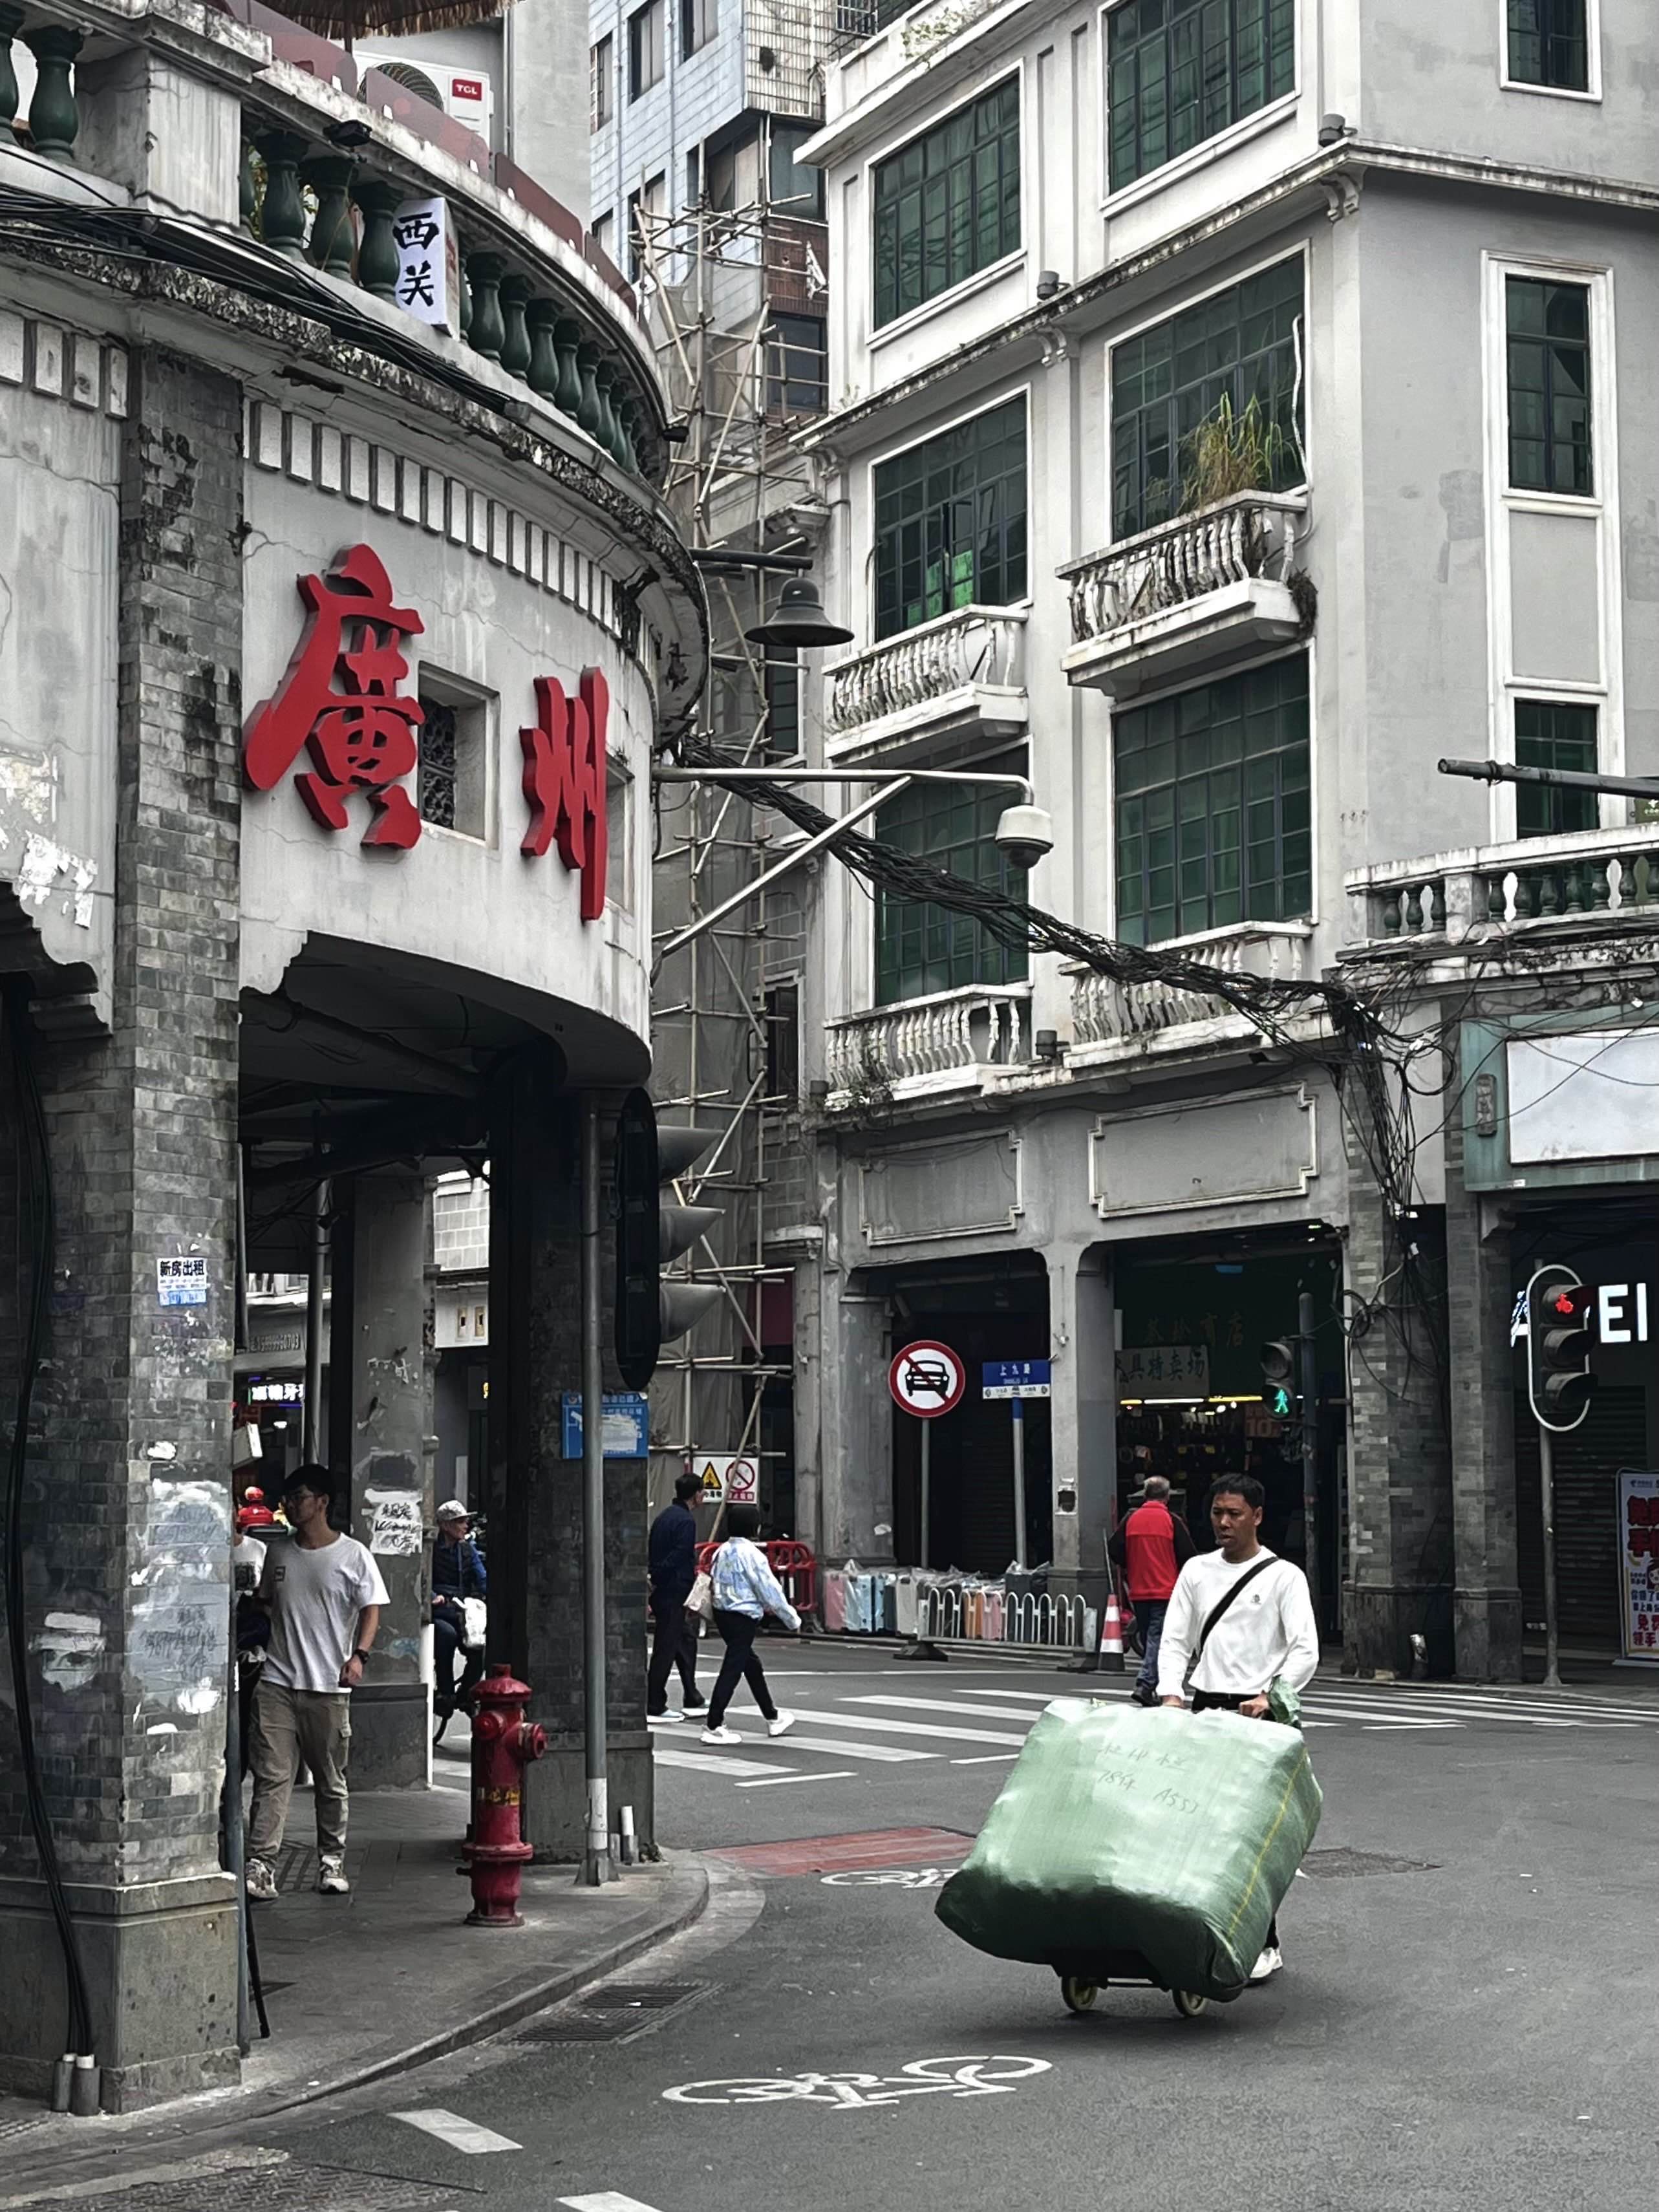
\includegraphics[scale=0.15]{GZXG}\\
\hfill\break
I will end the quarter with one of my favorite pictures taken in my hometown Guangzhou, China.\\ 
\end{center}

\hfill\break
\hfill\break
\noindent Thanks for reading this! Good luck on study, good luck on your exams, and good luck on your career! I hope you enjoy physics, and hope you have learned something from my worksheets :)\\



\end{document}
